\newpage
\subsubsection{Reasoning, Semantics, and Knowledge  Management}
\label{ict:modeling:kohlhase} \index{Kohlhase, Michael}

\paragraph{Research Team}
Michael Kohlhase (Professor),
Heinrich Stamerjohanns (Head of CS Labs, see~\ref{ict:stamer}),
Christoph Lange (PhD Student),
Christine M\"uller (PhD Student),
Normen M\"uller (PhD Student),
Immanuel Normann (PhD Student),
Florian Rabe (PhD Student),
Andrea Kohlhase (Research Programmer) \\

%%% give a very short (150 words description of your research area)
%% Hint: this can be copied from the research areas document (../masterplan/research-areas)

The ability to represent knowledge about the world and to draw logical inferences is one
of the central components of intelligent behavior, as a consequence, reasoning components
of some form are at the heart of many artificial intelligence systems.

The work of the KWARC (\underline{K}no\underline{w}ledge \underline{A}daptation and
\underline{R}easoning for \underline{C}ontent) group centers around building knowledge
management systems for e-science applications, in particular for the natural and
mathematical sciences.  The main assumption in this work is that if the structure of the
factual content of scientific documents, their contributions and dependencies regarding a
larger knowledge context is made sufficiently explicit, then this structure becomes
amenable to machine manipulation. Thus high-level added-value (web)-services can be offered,
e.g. semantic search and navigation (independent of the surface presentation),
user-adaptive presentation and content tailoring, and extended semantic quality control up
to proof verification.

\paragraph{Highlights}

%%% give a short (500 words)description of the research highlights. 1 figure costs 100 words
The highlight in 2006 was the publication of a 500 page book on OMDoc in the Springer
Lecture Notes in Artificial Intelligence series~\cite{Kohlhase:omdoc1.2}. OMDoc
({\underline{O}}pen {\underline{M}}athematical {\underline{Doc}}uments) is an
{\sc{Xml}}-based representation format for mathematical knowledge developed in the KWARC
group. This format is used in various ($\geq 10$) international projects as the knowledge
representation base.

\begin{figure}[ht]
\begin{center}
  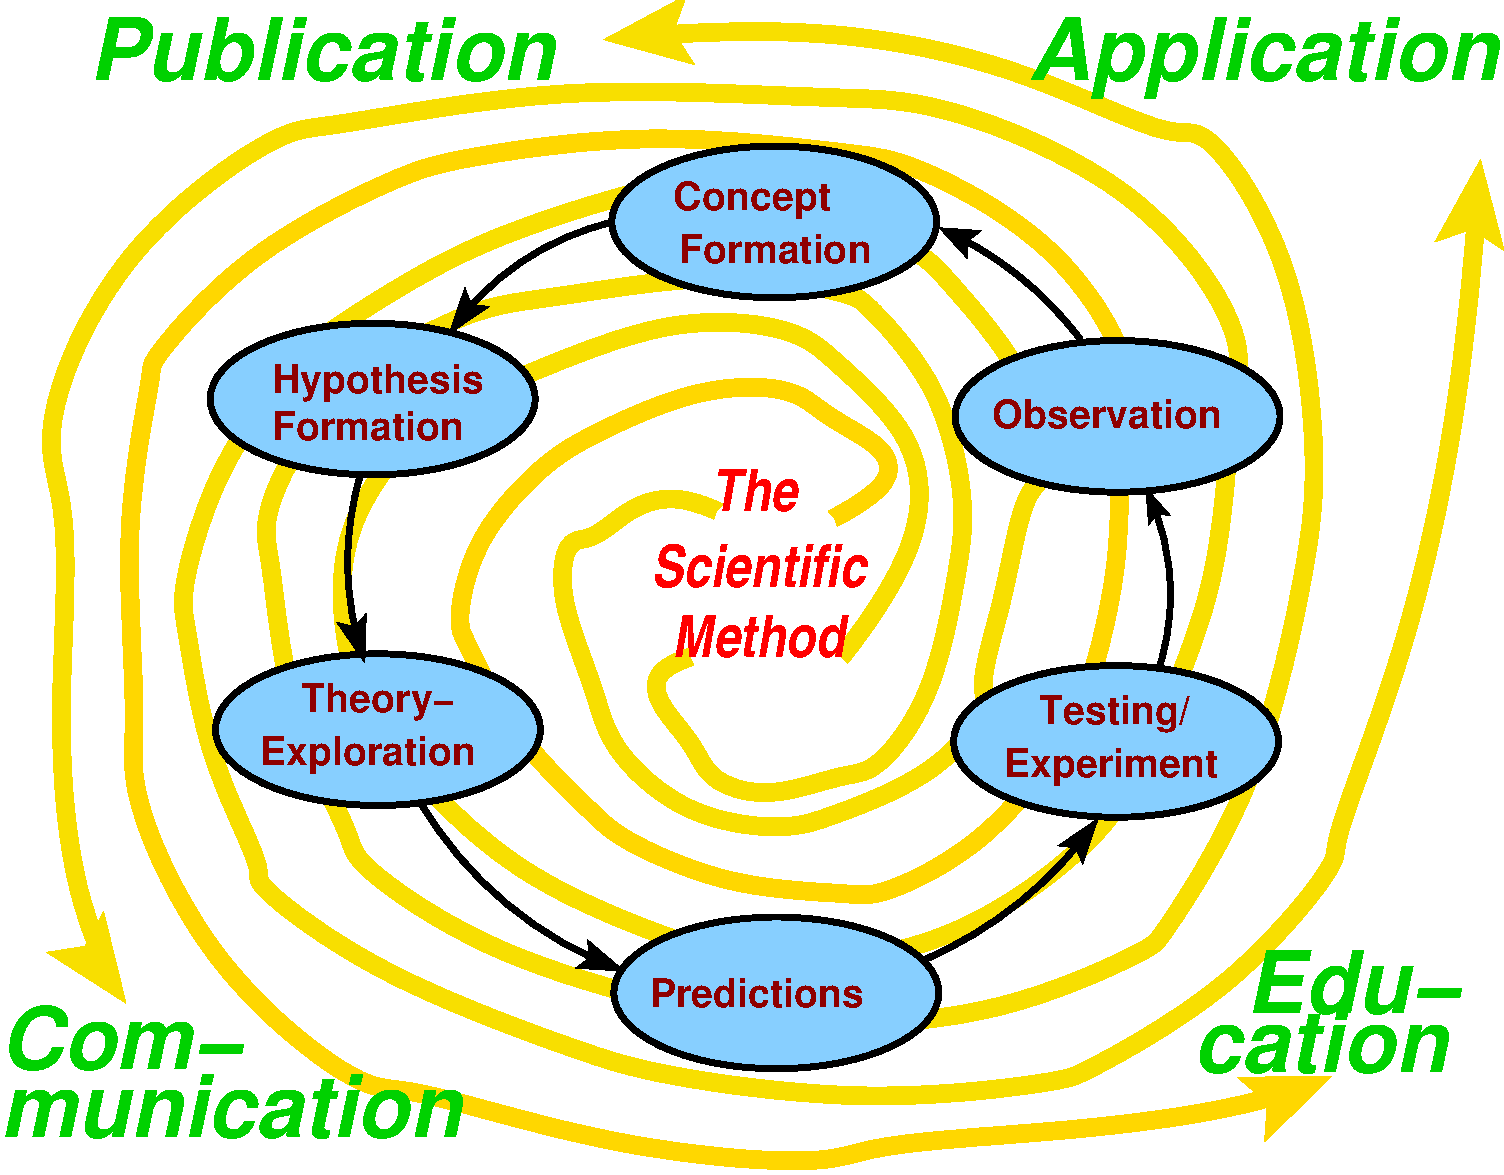
\includegraphics[width=7cm]{sci-method}
\end{center}
\caption{The Spiral View of Scientific Method}\label{fig:nw-Methode}
\end{figure}

We have extended the knowledge representation infrastructure in OMDoc to other topics in
the natural sciences to make it into a general semantic representation language that
supports seamless computer support in a ``{\emph{Scientific Semantic
    Web}}''~\cite{HilKohSta:copmem06}. Our starting point is the view of the
{\emph{scientific method}} as a spiral (Fig.~\ref{fig:nw-Methode}). In this view,
scientific research moves in a spiral trajectory from original ideas to results and
applications. At the moment, most of the steps in Fig.~\ref{fig:nw-Methode} are separately
supported by software systems, e.g. literature searches in Google Scholar or Wikipedia,
theory exploration in computer algebra systems and experiments in simulation systems. But
the systems are, largely, not able to inter-operate since they use differing data formats,
make differing model assumptions, and are bound to an implicitly given context that is
only documented in publications about the systems. A joint and universally applicable
representation language will be an enabling technology that alleviates these problems.

To make this vision come true, we have developed
\begin{enumerate}
\item a highly efficient, content-based document retrieval engine for
  mathematics~\cite{KohSuc:asemf06},
\item an OMDoc-based semantic WIKI~\cite{LanKoh:swim06,LanKoh:swmkm06,lange06:wikiblog},
\item a theoretical foundation for invasive editors and implementations in the MS Office
  suite~\cite{Kohlhase:UserAsPrisoner,Kohlhase:MediaOrMedeaSociety,Kohlhase:emPowerPoint},
\item methods for the discovery of theory morphisms in mathematical
  libraries~\cite{Normann:etrpti06}
\item a methodology for an ontology-based management of
  change~\cite{NRM:omdoc2vf06,Mueller06:locutor-lwa}, and
\item a representation format for logical systems with logic morphisms and
  proofs~\cite{rabe:dfol:06,rabe:moloss:06}
\end{enumerate}
We have started a research group of undergraduate CS students that undertake the
translation of the Cornell EPrint Archive from {\LaTeX} to XHTML+MathML (we can currently
translate 45\% of 400.000 articles in Physics, Mathematics, Computational Biology, and
Computer Science). This corpus will subjected of a semantic analysis with computational
linguistics methods and will be the basis of scalability studies for the methods and
representation formats presented above.

\paragraph{Organization}

In 2006, Prof. Michael Kohlhase was
\begin{enumerate}
\item Program and Conference Co-Chair of the 29.th Annual German Conference on Artificial
  Intelligence KI'06\cite{KI06}
\item Trustee of the Conference on Automated Deduction
\item Trustee of the Mathematical Knowledge Management Interest Group
\item Trustee of the CALCULEMUS Interest Group
\item Member of the Executive Committee of the OpenMath Society
\item Member of the MathML Working Group of the World Wide Web Consortium (W3C)
\item Member of 11 Program Committees of International Conferences.
\item Member of the Reviewer's College of the Engineering and Physical Sciences Review
  Research Council (EPSRC)
\item General Editor ``QPQ: an Online Journal for Peer-Reviewed Deductive Software
  Components'' {\url{http://www.qpq.org}}
\item Editor ``Journal of Applied Logic'', Elsevier.
\item Member of the ``Auswahlausschu\ss der Studienstiftung des Deutschen Volkes''
\end{enumerate}

\paragraph{Collaborations}
Prof. Michael Kohlhase is a Vice Director of the ``Safe and Secure Cognitive Systems'' of
the newly founded Department of the German Research Institute Lab Bremen. This leads to an
intensive collaboration of the KWARC group with this research group, which includes joint
projects and supervision of students. Further collaborations of the KWARC group include
\begin{enumerate}
    \item {\sl Rice University, USA}\\
          Prof. Richard Baraniuk\\
          Extending the Connexions Representation Format CNXML
    \item {\sl National Institute of Standards, USA}\\
          Dr. Bruce Miller\\
          Transforming {\LaTeX} documents to OMDoc/CNXML
    \item {\sl International University Bremen}\\
          Prof. Peter Baumann\\
          Extending OMDoc to GIS-Data/Living Documents
    \item {\sl Institute for Science Networking}\\
          Prof. Eberhard R. Hilf\\
          Extending OMDoc to PhysML
    \item {\sl Carnegie Mellon University, USA}\\
          Prof. Frank Pfenning, Prof. Peter Andrews\\
          Higher-Order Theorem Proving and Meta-Logical Frameworks
    \item {\sl Universit\"at des Saarlandes}\\
          Prof. J\"org Siekmann, Dr. Christoph Benzm\"uller\\
          Higher-Order Theorem Proving
    \item {\sl Deusches Forschungszentrum f\"ur K\"unstliche Intelligenz, Saarbr\"ucken}\\
          Dr. Dieter Hutter\\
          Ontology-based Management of Change
    \item {\sl Design Science Inc.}\\
          Dr. Robert Miner\\
          Mathematical Document Retrieval
\end{enumerate}

% \paragraph{Awards, Prizes}
% % list the awards, prizes you have received in 2005, if none have been received, plese delete this
% % subsection.
% \begin{enumerate}
% \item DAAD, grant for a year at Carnegie Mellon University.
% \end{enumerate}

\paragraph{Grants}
% list the running grants in 2005, if none have been received, please delete this
% subsection.
\begin{enumerate}
\item Funded by EU-IST (FP 6), \emph{ ONCE-CS}, (July 2005 -
December 2007)
\\
\item Funded by EU-IST (FP 6) \emph{JEM}, (July 2006 - July 2009)

%\item Industry: Design Science Inc. Grant for transforming Cornell Eprint archive.
\end{enumerate}

%\paragraph{Publications}
\nocite{BenBroKoh:csil06}
%\end{document}
%%% Local Variables:
%%% mode: latex
%%% TeX-master: "report"
%%% End:

% LocalWords:  Stamerjohanns EECS uller Normen Normann Rabe KWARC daptation Xml
% LocalWords:  easoning ontent OMDoc athematical uments Google Baraniuk CNXML
% LocalWords:  Baumann GIS Hilf Pfenning Universit des Saarlandes org Siekmann
% LocalWords:  Benzm Krieg uckner Deusches
